\documentclass{article}

\usepackage[utf8]{inputenc} %Only required if not using XeLatex
\usepackage[T1]{fontenc}
\usepackage[final]{microtype}
\usepackage{bm} %Bold font for math equations

\usepackage{helvet} %Set font type (helvetica)
\renewcommand{\familydefault}{phv} %Set helvetica as default font

\usepackage[a4paper]{geometry} %Setting document size and margin width

\usepackage{enumitem} %Custom list
\newlist{arrowlist}{itemize}{1} %Define custom list name
\setlist[arrowlist]{label=$\Rightarrow$} %Define arrow for custom list label

\usepackage{graphicx} %Required for graphics and figures
\graphicspath{./Fig/}
\usepackage[export]{adjustbox} %Used for adjusting image box
\usepackage{caption} %For caption customizations
\usepackage{subcaption}
\usepackage{float} %For [H] options of inserting figure

\usepackage[url=false, doi=false, isbn=false, bibstyle=ieee, citestyle=numeric-comp]{biblatex} %Set bibliography style (also error on compilation if not used)
\addbibresource{ref.bib} %Imports .bib file

\usepackage[breaklinks]{hyperref} %For url

\title{\textbf{Uncertainty Quantification of Plasma Filament in the Tokamak Scrape-off Layer}}
\author{Jasper Ng}
\date{May 2025}

\begin{document}

\maketitle

\noindent{\textbf{\Large Project Log}}

\begin{arrowlist}
    \item \textbf{Week starting from 02/04/2025}
    \begin{itemize}
        \item Discussed about the project specifics:
        \begin{itemize}
        	\item Premise of the project
        	\item Computational and physics aspects
            \begin{itemize}
        		\item[] Computational:
                \begin{itemize}
        			\item Use of Linux to compile C/C++ programmes
        			\item Use of Blob2d from BOUT++ framework
        			\item Use python for "gluing" everything together
                \end{itemize}
        		\item[] Physics:
                \begin{itemize}
        			\item Plasma filament occur in SOL of MCF fusion plasmas
        			\item Filaments created due to ExB forces
        			\item Blob size with different motions
                \end{itemize}
            \end{itemize}
        	\item Goals and objectives
        \end{itemize}
        \item Reading materials related to project
        \begin{itemize}
        	\item Plasma filament
        	\item Application of Gaussian process on tearing modes
        \end{itemize}
    \end{itemize}
    
    \item \textbf{Week starting from 04/03/2025}
    \begin{itemize}
        \item Discussion on Gaussian processes and specifics on components and methods:
        \begin{itemize}
        	\item Covariance matrix of multivariate Gaussian functions
        	\item Kernels for Gaussian processes
        \end{itemize}
        \item Risk assessment reviewed and submitted
    \end{itemize}
    
    \item \textbf{Week starting from 14/03/2025}
    \begin{itemize}
        \item Discussion on project specifics
        \begin{itemize}
        	\item Computational: Focus on environmental variables not numerical variables
        	\item Application of Gaussian process on plasma filament (blobs)
        \end{itemize}
        \item Version control training
    \end{itemize}
    
    \item \textbf{Week from 27/03/2025}
    \begin{itemize}
        \item Project objectives for the coming weeks
        \begin{itemize}
        	\item Install gcc on WSL
        	\item Compile BOUT++ and build programme
        	  \item Blob2d compiled and performed test runs
        	\item Create local and GitHub repository	
        	\item Create project log
        \end{itemize}
        \item Lay summary and Literature review
        \begin{itemize}
        	\item Deadline 08/05/2025
        	\item  Record literature in Zotero
        \end{itemize}
    \end{itemize}
    
    \item \textbf{Week from 15/04/2025}
    \begin{itemize}
        \item Discussion on coding specifics, and flags for compiling BOUT++ as well as running blob2d
        \begin{itemize}
            \item Record method of compilation such as use of cmake, and any flags/checks used
            \item Generally, less checks = faster runs, and checks include (refer to bout-dev build guide for checks):
            \begin{itemize}
                \item DCMAKE\_CXX\_FLAGS="-03"
                \item DBUILD\_TYPE=Debug
                \item DCHECK=0
            \end{itemize}
            \item Documentation for bout-dev: \url{https://bout-dev.readthedocs.io/en/latest/user_docs/quickstart.html#running-bout}
            \item Documentation for xbout module: \url{https://xbout.readthedocs.io/en/latest/index.html}, used for analysing results from BOUT++ runs
            \item For applying more cores for application run, use command "mpirun -n x" with x for amount of cores
            \item Github repository created to track project progress: \url{https://github.com/wxj512/Dissertation-Project.git}
        \end{itemize}
    \end{itemize}
    
    \begin{figure}[H]
    \centering
        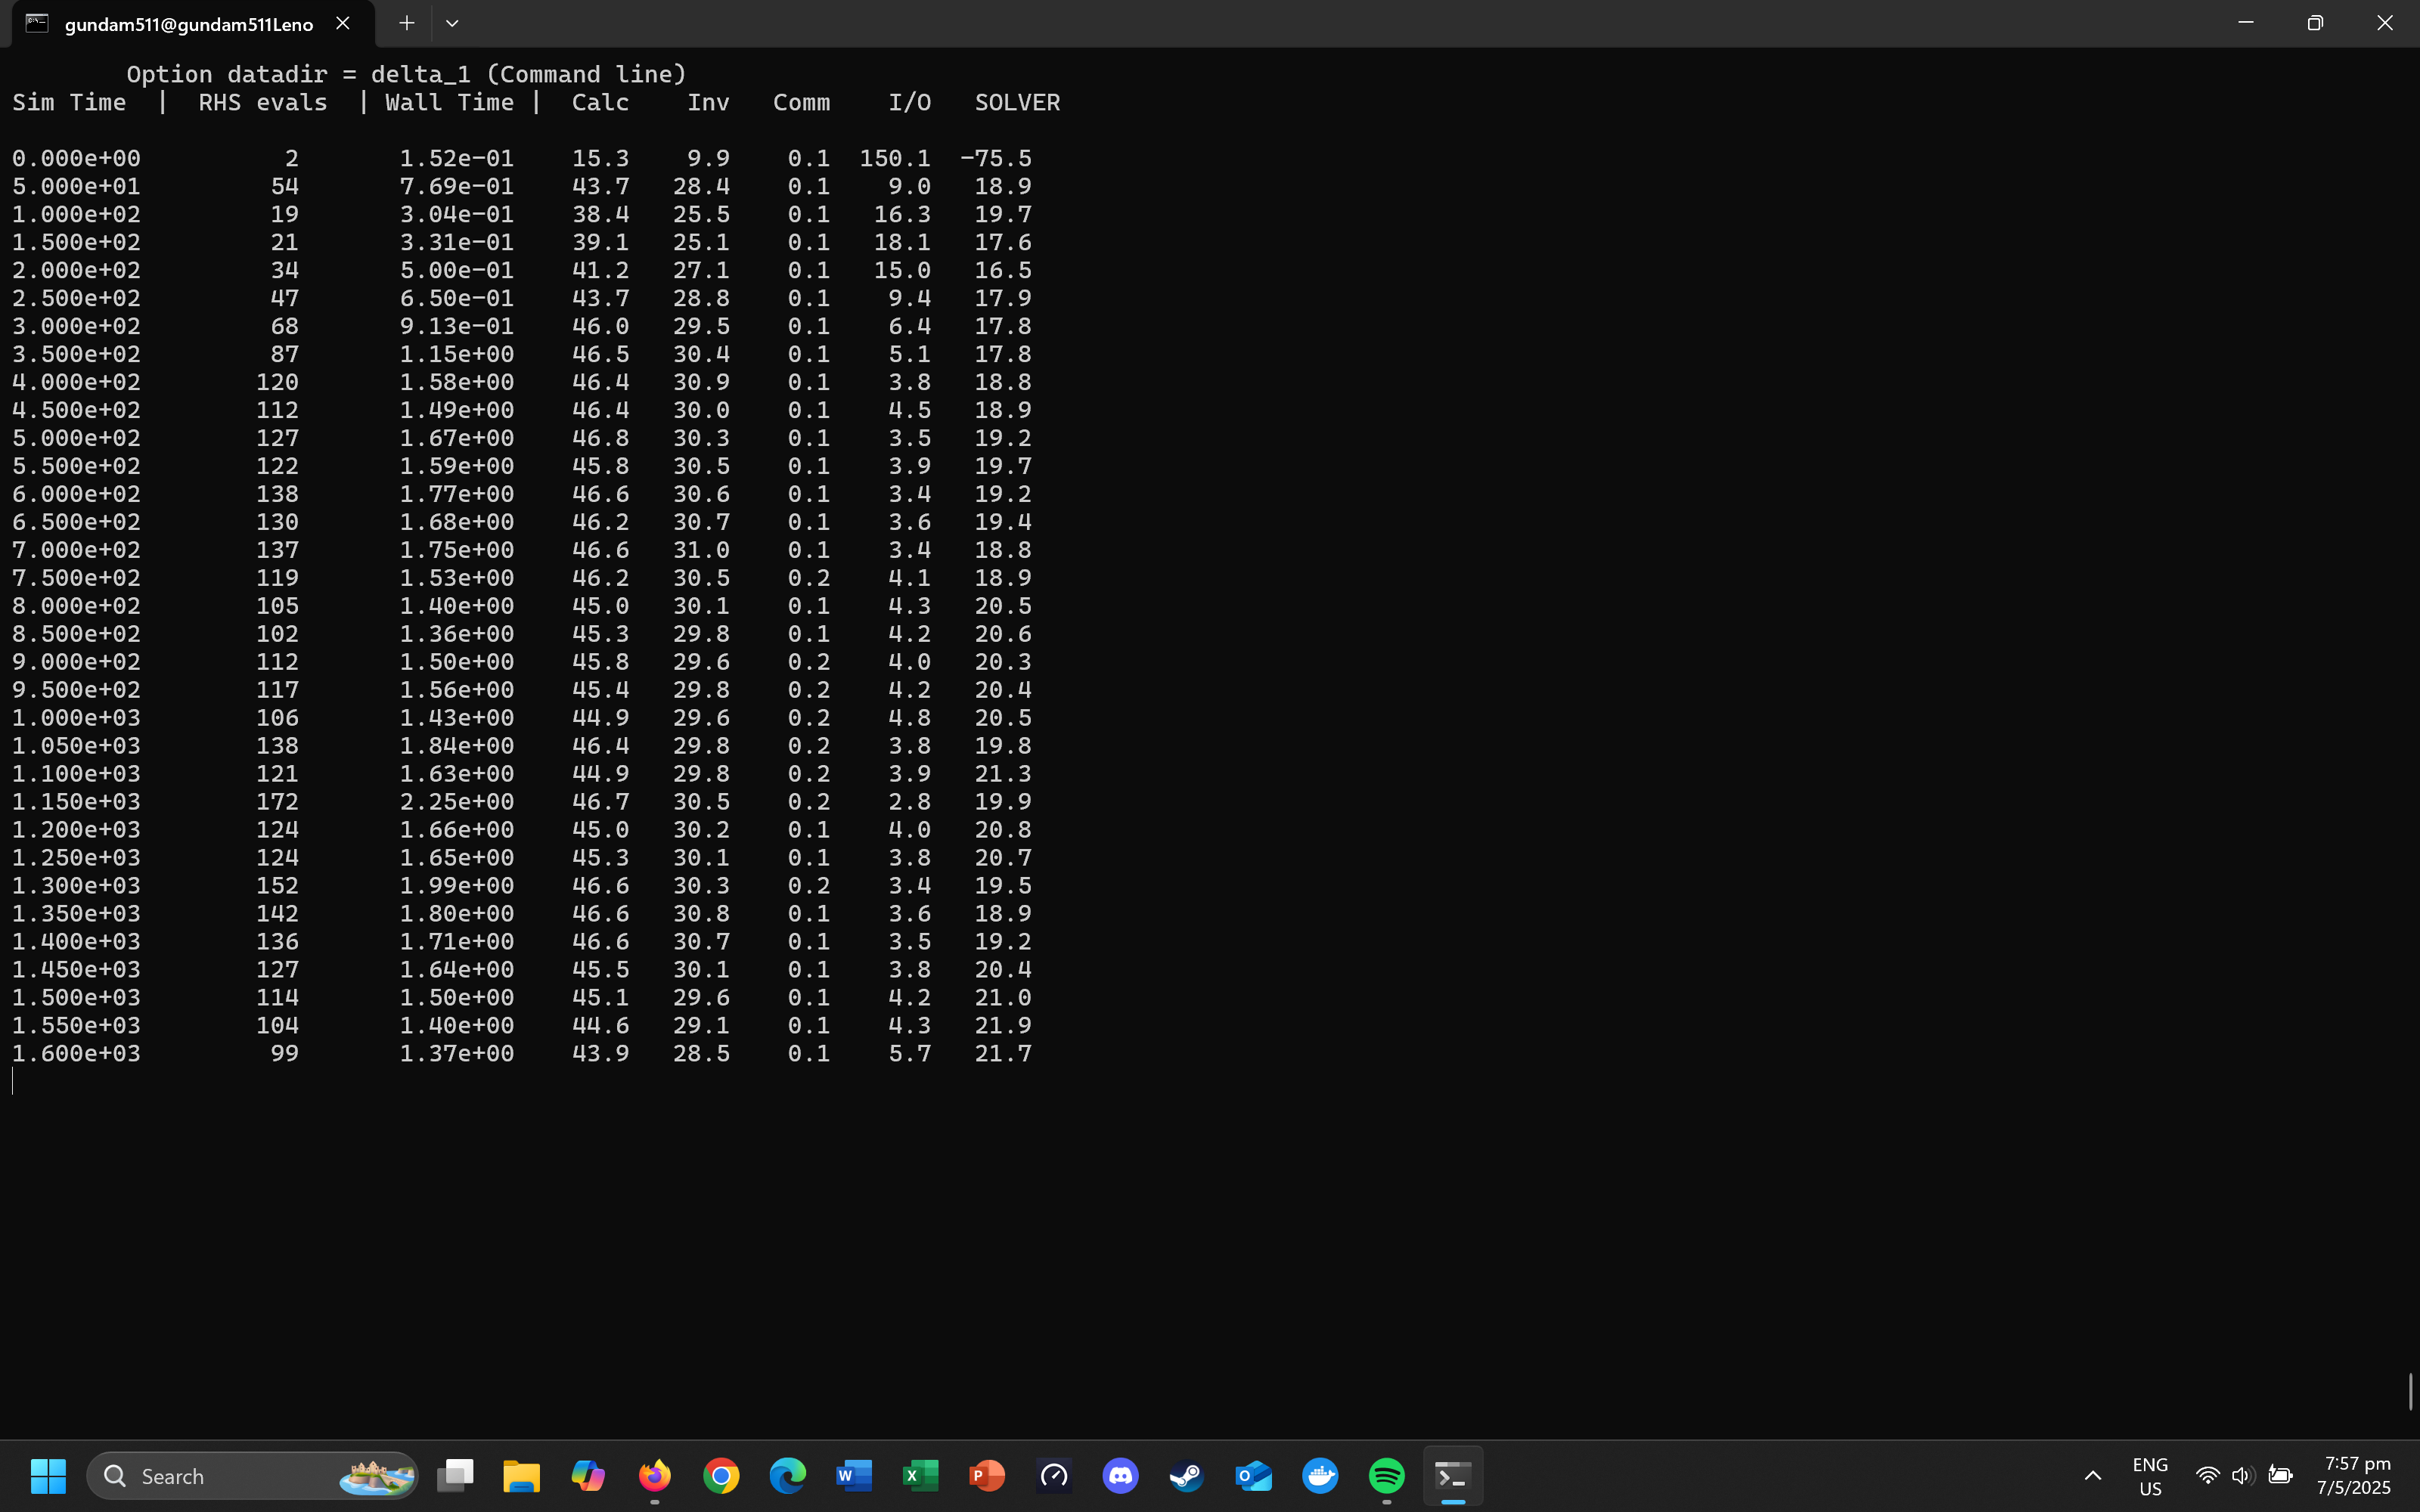
\includegraphics[height=0.3\textheight]{./Fig/Fig1 blob2d example run.png}
        \normalsize{\caption{Console view of blob2d run}
        \label{fig:fig1}}
    \end{figure}   

    \begin{figure}[H]
    \centering
        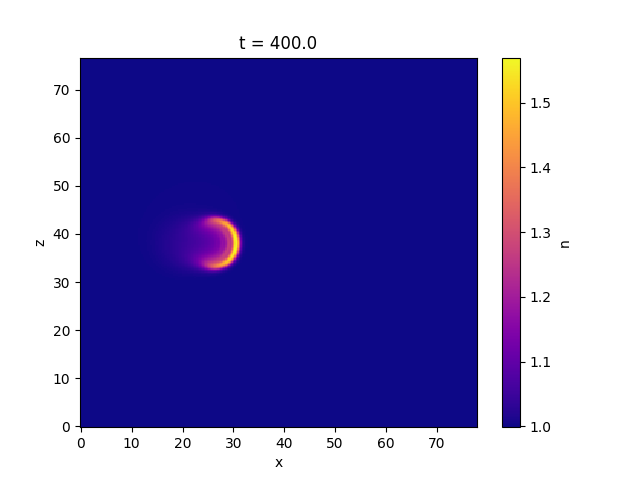
\includegraphics[height=0.5\textheight]{./Fig/Fig2 blob at t 400.png}
        \normalsize{\caption{Density (n) of blob at t=400s using input conditions from delta\_1 example}
        \label{fig:fig2}}
    \end{figure}   
    
    \item \textbf{Week from 29/04/2025}
       \begin{itemize}
            \item Drafted and finished literature review
            \item Refer to Lit\_rev\_plan.tex for details (could be found on Github repository)
       \end{itemize}

    \item \textbf{Week from 12/06/2025}
        \begin{itemize}
            \item Equations used in the blob2d simulation could be checked in the source file from BOUT-dev repository in BOUT-dev/examples/blob2d/blob2d.cxx
            \begin{itemize}
                \item Model (equations) solves and output density (n) and vorticity ($\Omega$) (equation taken from source file based on \cite{dudson_bout_2009}:
                \begin{itemize}
                    \item Base Equations:
                    \item[] $\frac{\partial n}{\partial t}=-\left[\phi,n\right]+2\frac{\rho_s}{R_c}\frac{\partial n}{\partial z}+D_n{\nabla^2_{\perp}}n$
                    \item[] $\frac{\partial \Omega}{\partial t}=-\left[\phi,\Omega\right]+\frac{2}{n}\frac{\rho_s}{R_c}\frac{\partial n}{\partial z}+\frac{1}{n}D_{\Omega}{\nabla^2_{\perp}}{\Omega}$
                    \item Compressible $E\times B$ term option:
                    \item [] (For $\frac{\partial n}{\partial t}$) Add $-2n\frac{\partial \phi}{\partial z}\frac{\rho_s}{R_c}$
                    \item Sheath closure option:
                    \item [] (For $\frac{\partial n}{\partial t}$) Add $n\phi\frac{\rho_s}{L_{\parallel}}$
                    \item [] (For $\frac{\partial \Omega}{\partial t}$) Add $\phi\frac{\rho_s}{L_{\parallel}}$
                \end{itemize}
                \item Output variables are normalised and scaled to $1\times 10^{-19}$
            \end{itemize}
            \item With reference to \cite{omotani_effects_2015} input parameters could change velocity of blob. Since this project is revolved around uncertainty quantification of plasma filament, input parameters that would affect the output would have to be defined. However, as shown above, model only outputs n and $\Omega$, hence velocity would have to be calculated.
            \begin{itemize}
                \item Velocity of the 'blob' could be defined by the distance moved within the time frame of simulation: 
                \begin{equation}\label{V_f_eqn}
                    V_f=\frac{dx}{dt}
                \end{equation}
                \item To define the distance (x) moved for the blob, the centre of mass (CoM) of the blob would have to be defined in order to calculate the overall movement of the blob within the grid
                \item Since the model uses a coordinated grid to solve for n and $\Omega$ the CoM is the weighted average of the density distribution of the grid:
                \item[] \[ \sum_{i=1}^{N} \left(c_{i(x,z)}-c_{CoM(x,z)}\right)\times n_i \]
                \begin{equation}
                    c_{CoM(x,z)}=\frac{\sum_{i=1}^{N} n_ic_{i(x,z)}}{\sum_{i=1}^{N} ni}
                \end{equation} 
                \item where N is the number of points of the grid, c represents the coordinate (x or z for the blob2d model) and n is the density of the blob at each time interval of the simulation
                \item The CoM at each time interval of the simulation is found and using the known time difference at each time interval, the velocity is found by using (\ref{V_f_eqn}) and dividing the change in CoM by the time difference (or the gradient of the CoM array)
                \item Distance/velocity could be calculated for each individual coordinate, or as an euclidean distance between 2 points of CoM for each pair of time intervals
                \item For the delta\_1 example case (Found in BOUT++ repository: \url {https://github.com/boutproject/BOUT-dev/tree/master/examples/blob2d}), the time difference for each interval is 50, and the grid size for both coordinates (dx or dz) is 0.3
                \item The CoM is found using the center\_of\_mass module from scipy and the gradient and linalg.norm module from numpy and the full python file for processing could be found in the github repository of the project (\url{https://github.com/wxj512/Dissertation-Project.git} in Misc/Test/Scripts/v\_data.py)
            \end{itemize}  
       \end{itemize}

    \begin{figure}[H]
    \centering
        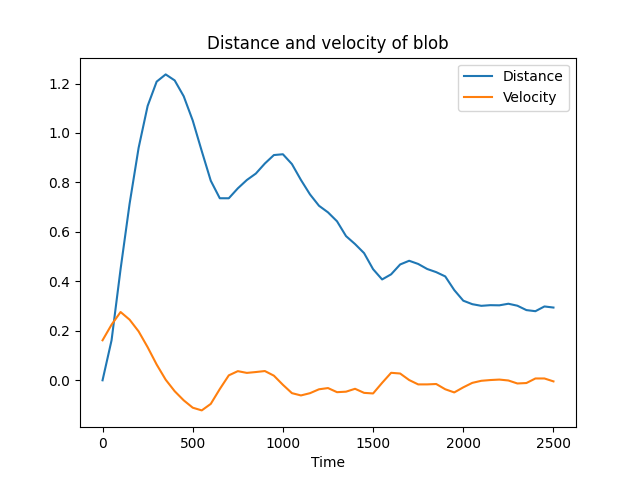
\includegraphics[height=0.5\textheight]{./Fig/Fig3 vel plot.png}
        \normalsize{\caption{Velocity and Distance plot for delta\_1 example}
        \label{fig:fig3}}
    \end{figure}   

    \item \textbf{Correction and Supplement to Week from 12/06/2025}
    \begin{itemize}
        \item For reference of the python file for processing, in addition to the file location provided, the commit hash of the file is 628ecbf
        \item For Figure \ref{fig:fig3}: Figure is updated to Figure \ref{fig:fig4} below to give proper labels for axis. Time is normalised to the inverse of cyclotron frquency ($1/\Omega_i$), distance is normalised to Bohm gyro radius ($\rho_s$) and velocity is normalised to Bohm sound speed ($c_s$). Default units were taken from blob2d.cxx source file and BOUT.inp from delta\_1 folder (Found in BOUT++ repository: \url{https://github.com/boutproject/BOUT-dev/tree/master/examples/blob2d}) 
    \end{itemize}

    \begin{figure}[H]
    \centering
        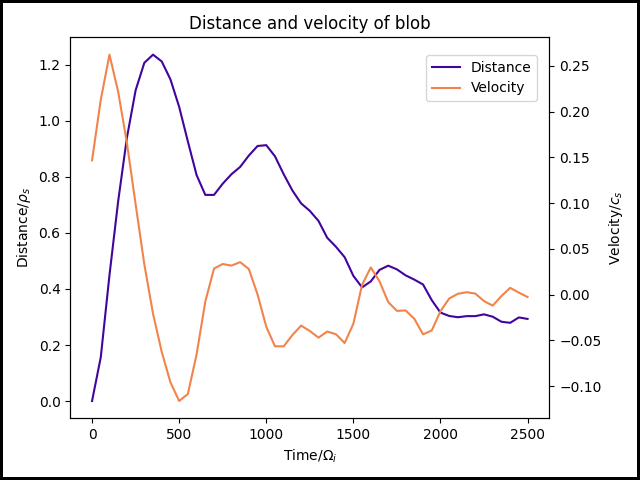
\includegraphics[height=0.5\textheight]{./Fig/Fig3 vel plot_v2.png}
        \normalsize{\caption{Velocity and Distance plot for delta\_1 example}
        \label{fig:fig4}}
    \end{figure}   

\item \textbf{Correction to Figure 4}
    \begin{itemize}
        \item For Figure \ref{fig:fig4}: Figure is updated to Figure \ref{fig:fig5} below to correct the units for time as 1/$\Omega_i$ and supplemented velocity calculation method in caption
    \end{itemize}

    \begin{figure}[H]
    \centering
        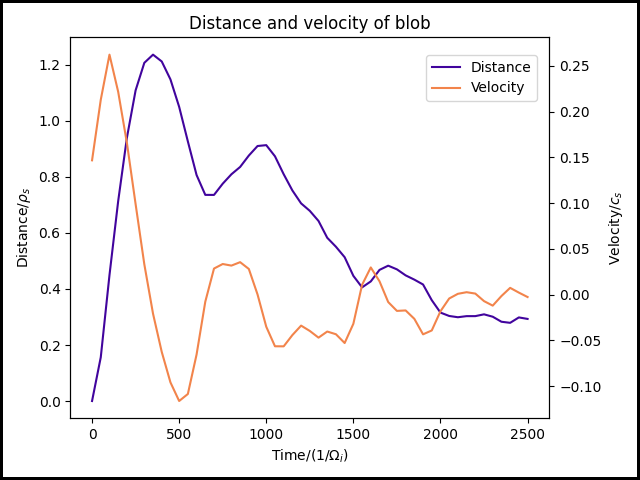
\includegraphics[height=0.5\textheight]{./Fig/Fig3 vel plot_v3.png}
        \normalsize{\caption{Velocity and Distance plot for delta\_1 example using Centre of Mass (CoM) method}
        \label{fig:fig5}}
    \end{figure}   

    \item \textbf{Week from 19/06/2025}
        \begin{itemize}
            \item 2 other methods for velocity calculation were proposed, which calculates velocity by evaluating the position of maximum density (max n) for the blob, and the position of the density front (n front) of the blob
            \item Some errors still remain for distance and velocity for the CoM method from previous week, therefore CoM method would be corrected and supplemented below
            \item All method comparisons were done using the delta\_1 example mentioned previously (Found in BOUT++ repository: \url{https://github.com/boutproject/BOUT-dev/tree/master/examples/blob2d}) and Figure \ref{fig:fig6} below shows the density evolution of the blob for 0 to 2500 (1/$\Omega_i$) in intervals of 500 (1/$\Omega_i$)
            \item The euclidean distance and velocity was not calculated for the methods as the variation in the z direction is minimal and not applicable to some methods
            \item Latest version of the file could be found at 

    \begin{figure}[H]
    \centering
        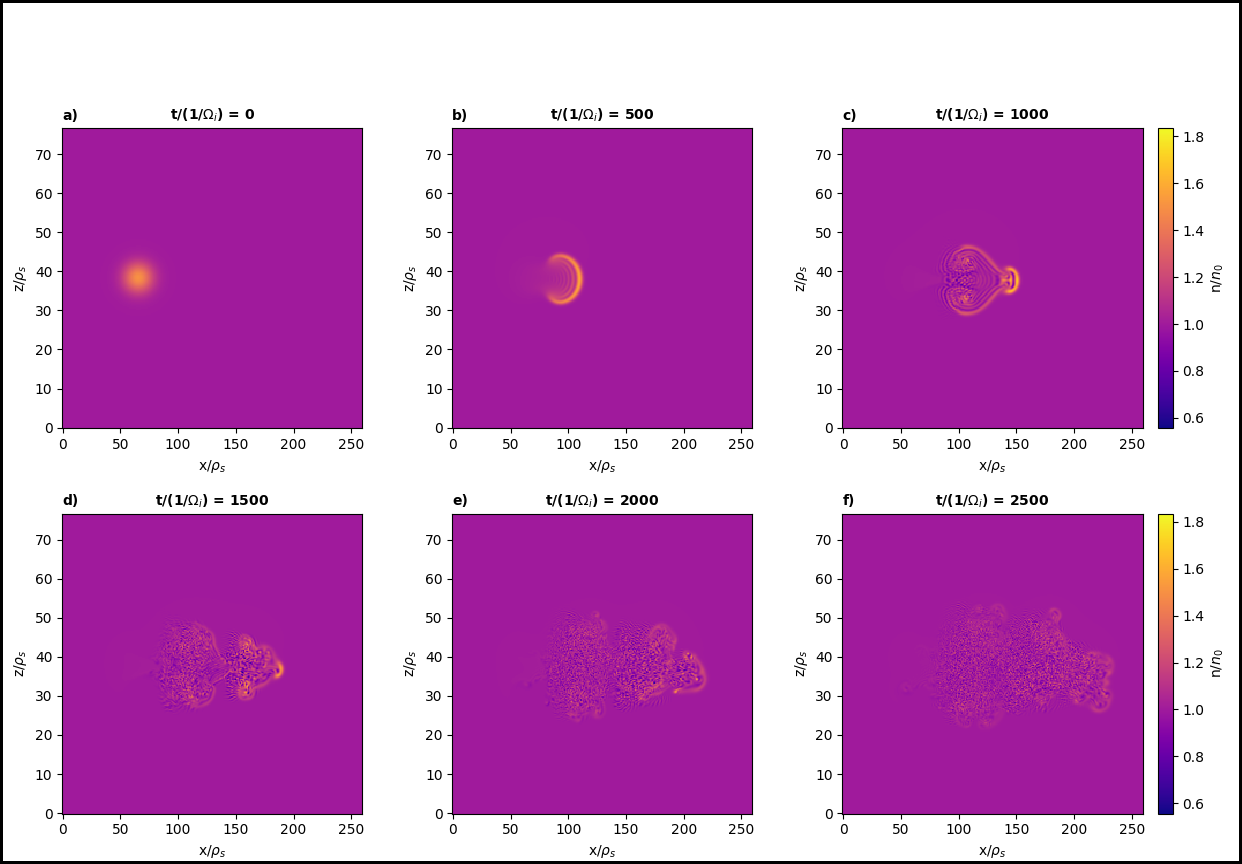
\includegraphics[height=0.5\textheight]{./Fig/Fig6 n hmap t0_t50}
        \normalsize{\caption{Density evolution of blob for delta\_1 example at different t/(1/$\Omega_i$): a) 0 b) 500 c) 1000 d) 1500 e) 2000 f) 2500. By d) it could be shown that the blob has lost symmetry and the density of the blob is dispersed. The colour of the blob (such as the yellow dot at a), showing regions of high density compared to the background density $n_0$) becomes very similar to the background, showing the blob density (n) is much closer to the background density ($n_0$) and the value of n/$n_0$ is close to 1 as time evolves}
        \label{fig:fig6}}
    \end{figure}   
            
            \item \textbf{CoM method}
            \begin{itemize}
                \item As mentioned previously CoM method computes the CoM for the density of the grid for each time slice to evaluate the distance travelled and velocity of the blob
                \item The point of CoM are overlaid onto the density plot of the blob for different times to show the CoM evolution of the blob that were used to evaluate the distance and velocity, shown below in Figure \ref{fig:fig7}
                \item The CoM method of calculation for distance and velocity as shown in Figures \ref{fig:fig3}, \ref{fig:fig4} and \ref{fig:fig5} were actually the velocity and acceleration instead, hence the figure is replotted and shown below in Figure \ref{fig:fig8} below
                \item Latest version for the python file to calculate CoM method could be found at project repository (\url{https://github.com/wxj512/Dissertation-Project.git} in Misc/Test/Scripts/v\_data.py commit number 9813f1e)  

    \begin{figure}
        \centering
        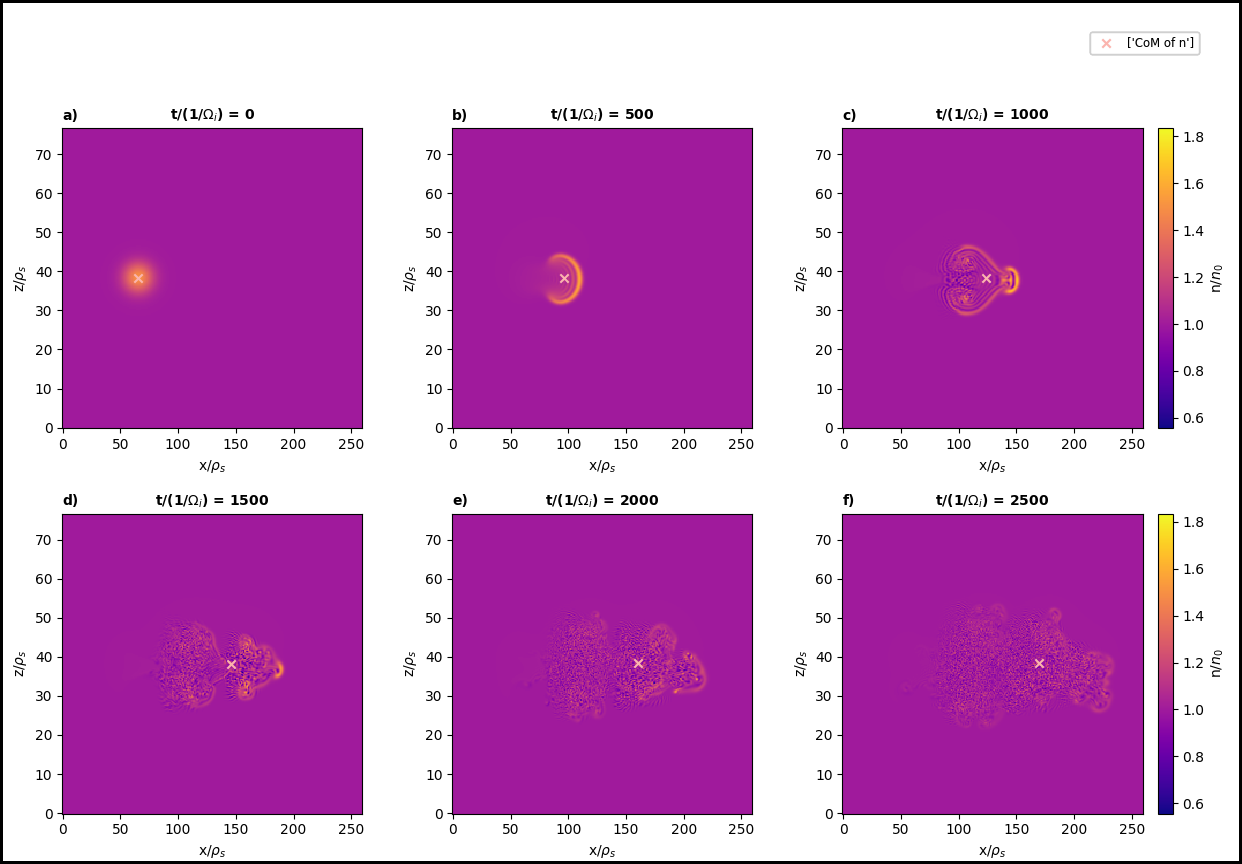
\includegraphics[height=0.5\textheight]{./Fig/Fig7 vel n CoM hmap t0_t50}
        \normalsize{\caption{CoM for blob density at different t/(1/$\Omega_i$) depicted as "x" overlaid on density evolution of blob for delta\_1 example at different t/(1/$\Omega_i$): a) 0 b) 500 c) 1000 d) 1500 e) 2000 f) 2500. As the blob starts to disperse after a) the CoM point is further away from the density front of the blob and closer to the centre of the blob area in d) to f) as the density is evenly dispersed into nearby space}
        \label{fig:fig7}}
    \end{figure}   

   \begin{figure}[H]
        \centering
        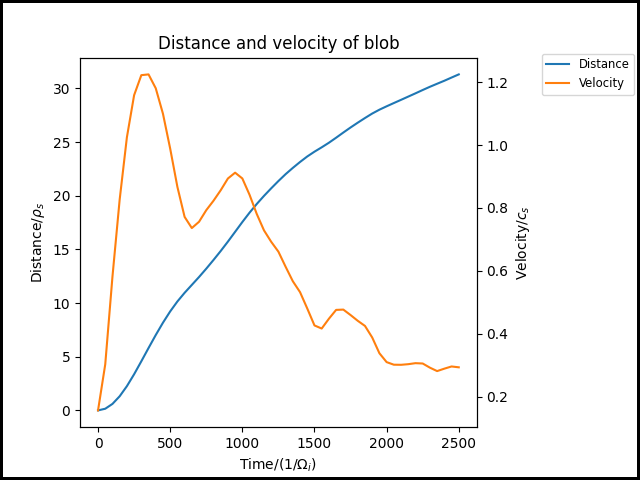
\includegraphics[height=0.5\textheight]{./Fig/Fig8 CoM dist vel plot.png}
        \normalsize{\caption{Distance (blue line) and velocity (orange line) of the blob in the x direction from delta\_1 example as calculated using CoM method}
        \label{fig:fig8}}
    \end{figure}  
    
                \item As the blob moves in the positive x direction, the distance increases as shown in Figure \ref{fig:fig8}, but as depicted in Figure \ref{fig:fig7} that the blob disperses and the CoM are closer to the centre of the area of the blob instead of the front
                \item Since the blob is dispersed the area of the blob is stretched in both x and z direction, with more elongation in the x direction, causing the blob front in the x direction to be further away from the point of CoM than the z direction 
            \end{itemize}

            \item \textbf{n front method (peak and FWHM)}
            \begin{itemize}
                \item n front method calculates the distance by locating the "density front" of the blob using the last "density peak" in the x direction
                \item Density peaks are found by taking the density profile of the blob at a row for each time value and finding the x value of where the density peaks, and the peaks could be evaluated with only the mid row of z, or for all rows of z
                \item The peak position with the largest x coordinate value corresponding to the peak density values (mid row or after evaluating all the rows of z) is determined to be the density front of the blob, 
                \item For each row of density data to be evaluated the peak in the density is found using find\_peaks module from Scipy 
                
    \begin{figure}[H]
        \centering
        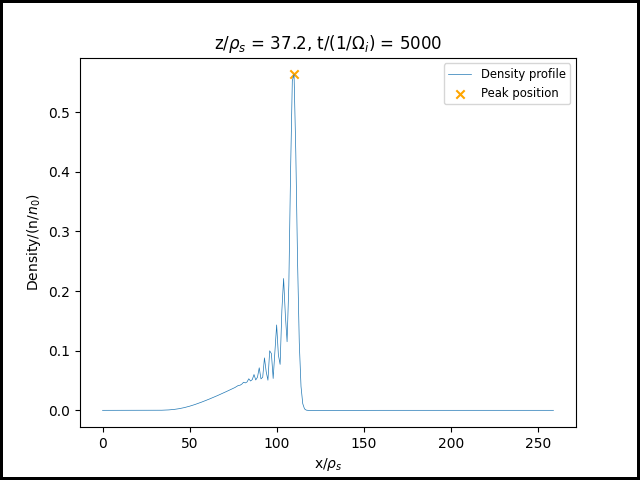
\includegraphics[height=0.5\textheight]{./Fig/Fig9 n front n peak plot.png}
        \normalsize{\caption{Density profile (blue line) and peak position (orange "x") for density of blob at mid row of z and t/(1/$\Omega_i$) at 5000}
        \label{fig:fig9}}
    \end{figure}  
    
                \item Additionally a gaussian peak could be fitted over the peak and the x position of the right side of the full width at half maximum (FWHM) of the gaussian function could be 
                defined
                \item The gaussian distribution function has the following form \cite{chirikjian_gaussian_2009}:
                \item[] \[ A\exp{-\left(\frac{\left(x-\mu\right)^2}{2\sigma^2}\right)} \]
                \item[] \[ A = \frac{1}{\sqrt{2\pi}\sigma}=s\]
                \item where s is the spread (corresponding to height of gaussian function and the density at the peak position), $\mu$ is the mean (or in this case the x coordinate of the peak) and $\sigma^2$ is the variance of the distribution 
                \item The operation of fitting a gaussian function over the peak of the density assumes it has a gaussian distribution for that particular peak
                \item The FWHM was used as it could characterize the width of a peak that resembles a gaussian function, and has the following form \cite{rainio_methods_2025}:
                \item[] \[ FWHM = \sqrt{8\ln{2}}\sigma \]
                \item where $\sigma$ relates to the variance of the gaussian function
                \item An example for one of the the gaussian fit is shown below in Figure \ref{fig:fig10}

    \begin{figure}[H]
        \centering
        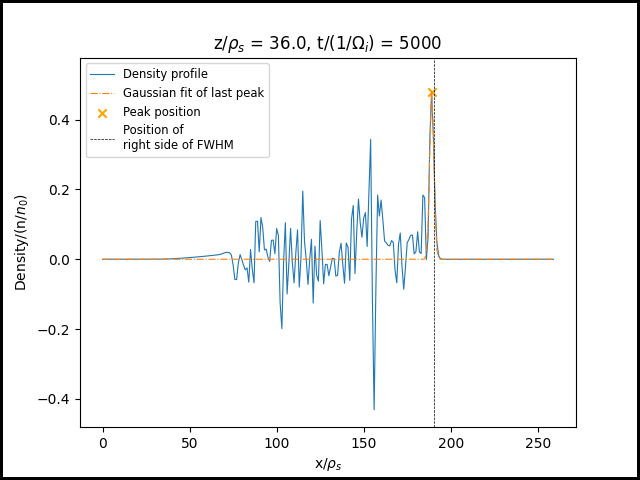
\includegraphics[height=0.5\textheight]{./Fig/Fig10 n front FWHM plot.png}
        \normalsize{\caption{Density profile (blue line), peak position (orange "x") for density of blob and gaussian function fit (orange dash-dot line) and right position of FWHM for the gaussian fit (black dotted line) at z/$\rho_s$ at 36 and t/(1/$\Omega_i$) at 15000}
        \label{fig:fig10}}
    \end{figure}  
                
            \end{itemize}
            
            \item CoM method displayed the wrong distance, replotted here
            \item n\_calc methods: n front and max n
            \item max n no feasible as blob disperses and max n does not track the "front" and distance move backwards due to dispersed blob (both mid-plane row and all rows)
            \item n front is possible but finding the row that has the furthest front could take a long time (~1:58), and adding FWHM does not vary simulation time significantly
        \end{itemize}
    
\end{arrowlist}



\nocite{*}
\printbibliography[title={References}]

\end{document}